\documentclass[11pt]{article}

\usepackage{graphicx}
\usepackage{algorithmic}
\usepackage{algorithm}



\newcommand {\Real}{\mathrm{R}}



\title{Climate deviation model estimation with Kalman filter}

\author{Julio Waissman Vilanova}\date{}

\begin{document}

\maketitle

\section{The climate deviation model strategy}

Let $P_{ij}(t)$ and $L_{ij}(t)$ the observed precipitation and lighting gaussian counts in
grid $i,j$ at time $t$ respectively. The aim of the model is to estimate the precipitation
$\hat{P}_{ij}(t)$ using the lightning data at the current  grid  $i,j$ and space and time
vicinity. The $\hat{P}_{ij}(t)$ is estimated at two stages: the frist stage using a
linear space and time invariant seasonal model (STI) adjusted by a least square
methodology and the second, a climate
deviation model (CD) adjusted dynamically by means of a Kalman filter. 
The general scheme is shown in figure 1.

\begin{center} 
  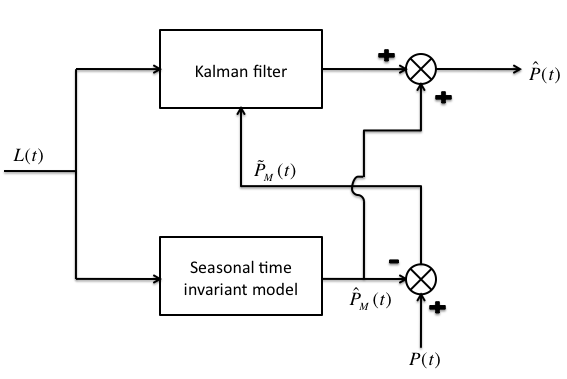
\includegraphics[width = 0.9\textwidth]{scheme.png}  

Figure 1: The big picture
\end{center}


Let $L(t)$ be a vector of lightning for all the
grids of the region of interest in the form
$$
L(t) = (L_{11}(t), L_{21}(t), ldots, L_{N1}(t), \ldots L_{ij}(t), \ldots, L_{NM}(t))^T,
$$
where $M$ is the number of grid rows and $N$ the number of grid columns. With the STI
model, a model precipitation estimation of all the grids is obtained $\hat{P}_M(t)$ like a
vector similar to $L(t)$. {\bf In fact, not only $L(t)$ is used, but also $L(t-nl),
  \ldots, L(t+np)$ but i don´t know yet how to express that in a clear form in the scheme}.

The prediction made by the STI model is sustraed to the observed precipitation vector
$P(t)$ resulting a error estimation vector $\acute{P}(t)$. The main idea is to develop an
estimation system in order to adjust a Climate Deviation Model to estimate the deviation
of the seasonal model of the STI estimation. The predicted deviation is then adding to the
$\hat{PM}(t)$ in order to obtain a corrected estimated precipitation $\hat{P}(t)$. 

Let $nb_V(L_{ij}(t))$ the vector of spatial $V$ neighborhood  
$$
nb_V(L_{ij}(t)) = (L_{i-V,,j-V}(t), \ldots, L_{i,j-V}(t), \ldots, L_{i,j}(t), \ldots, L_{i+V,j+V}(t))^T)^T,
$$
and let $\Lambda_{i,j}(t)$ the vector
$$
\Lambda_{ij}(t) = (nb_V(L_{ij}(t-nl)^T, \dots, nb_V(L_{ij}(t+pl)^T, 1 )^T,
$$ 
where $nl$ are de number of negative lags and $pl$ the number of positive lags considered
in the STI model.

Then, the $\hat{P}M_{ij}(t)$ is obtained as
$$
\hat{P}M_{ij}(t) = \Lambda_{ij}(t)^T \Theta
$$
where $\Theta = (\theta_1, \ldots, \theta_k, b)$ is the parameter vector for linear
regression. In order to compute $\Theta$ all the grids of the season marked as convective
grid are used in a classical least squares algorithm.

The STI model is static and reflect the general tendency of the season. Thus, a Climate
Deviation dynamical model can take in account the diferences along the season. It is important to
notice that the CD model only take in account the variation in time of the STI model,
because we use one set of parameters for all the grids of the region at time $t$. 

The CD model is assumed with the same neighborhood $V$ and the same positive and negative
lags of the STI model. {\bf I don't  know if it is a good idea, because if we consider
  positive lags in the dynamical model, then we assume that we have the $L(t+1), \ldots
  L(t+pl)$ data available, and then we can not argue that the model is useful to doing
  nowcasting}.

The CD model is then a model of the diferences between the estimation of the STI model
respect the observed data at time $t$, 
$$
\hat{D}_{ij}(t) = \Lambda_{ij}(t)^T \Phi(t)
$$
where $\Phi(t) = (\phi_1(t), \ldots, \phi_k(t), \beta(t))^T$ is the vector of dynamical
parámeters of the CD model and $\hat{D}_{ij}(t)$ is the precipitation deviation at time
$t$ for the grid $i,j$.. The model can be represented with a matrix notation in order
to obtain the vector of the deviation of entry region at time $t$ as
$$
D(t) = \Lambda(t) \Phi(t)
$$ 
where
$$
\Lambda(t) = \left[
  \begin{array}[c]{c}
    \Lambda_{11}(t)^T \\
    \vdots \\
    \Lambda_{ij}(t)^T \\
    \vdots
    \Lambda_{NM}^T
  \end{array}
\right]
$$

The Kalman algoritm used in this work is

\begin{algorithm} 
\caption{General CD Kalman filter procedure} 
\begin{algorithmic}[1]
\REQUIRE $\Theta$
\REQUIRE $H$ matrix of coverture (\emph{not explained yet})
\REQUIRE $Q$ covariance matrix of the CD model parámeters uncertainty
\REQUIRE $R$ covariance matrix of the gaussian white noise in measurements
\REQUIRE $\tau$ parameters' decay time constant
\REQUIRE $h$ an int to decide that Precip with no Lightning is far enough 
\REQUIRE $A(0)$ \emph{a posteriori} error covariance matrix
\STATE $\alpha \leftarrow 0$
\STATE $\Phi(0) \leftarrow (0, 0, \ldots, 0)^T$

\FOR{$t$ from $ln+1$ to $t_f - lp$ }
           \STATE Read Lightning data to form $\Lambda (t)$
           \IF{ all entries of $\Lambda(t)$ are zero}
                     \STATE $\hat{P}M(t) \leftarrow [0, \ldots, 0]]$
           \ELSE
                      \STATE $\hat{P}M(t) \leftarrow \Lambda(t) \Theta$
           \ENDIF
           \IF{(zero convective grid in all the region at times $t-nl, \ldots, t+pl$ \AND
             $P(t)$ have at least one entry different from zero) \OR ($P(t-h), \ldots,
             P(t)$ dont have any entry different from zero)}
                      \STATE $\Phi(t) \leftarrow \Phi(t-1) \exp(-\alpha \tau)$
                      \STATE $\alpha \leftarrow \alpha + 1$
                      \IF{ $\alpha \ge \frac{3}{\tau}$}
                                   \STATE $A(t) \leftarrow A(0)$
                      \ENDIF
           \ELSIF{$P(t)$ have at least one entry different from zero}
                      \STATE $\alpha \leftarrow 0$
                      \STATE $A(t) \leftarrow A(t-1) + Q$
                      \STATE $C \leftarrow H \Lambda(t)$
                      \STATE $K \leftarrow A(t) C^T (C A(t) C + R)^{-1}$ 
                      \STATE $E \leftarrow H P(t) - C\Phi(t) $
                      \STATE $A(t) \leftarrow (I - KC)A(t)$
                      \STATE $\Phi(t) \leftarrow K \Phi(t-1)$ 
          \ENDIF
          \STATE $D(t) \leftarrow \Lambda(t) \Phi(t)$
          \STATE $\hat{P}(t) \leftarrow \hat{P}M(t) + D(t)$
\ENDFOR
\ENSURE $\hat{P}(t)$

\end{algorithmic}
\end{algorithm}

\end{document}

